\section{Experiments}
\subsection{Experimental Setup}
\label{sec:exp}
\noindent \textbf{Benchmarks.}
We evaluate the effectiveness of the Info-Gain Sampler on diverse settings:
(1) Fully-Attention MDM Reasoning:
Math (GSM8K, MATH-500; 0-shot)~\cite{cobbe2021gsm8k,hendrycksmath2021},
Code (HumanEval, MBPP; 0-shot)~\cite{chen2021evaluating,austin2021program},
and Planning (4$\times$4 Sudoku; 5-shot~\cite{qin2025backtrack}, Countdown; 3-shot with 3 numbers~\cite{ye2025dream}),
reporting average Pass@1 accuracy over 5 runs;
{(2) Semi-Autoregressive MDM Reasoning:}
evaluated on the same Math and Code benchmarks
in a zero-shot setting, reporting average Pass@1 accuracy over 5 runs;
{(3) Multimodal Text-to-Image Generation:}
evaluated on ImageNet-512 and GenEval~\cite{ghosh2023geneval},
with IS~\cite{salimans2016improved}, FID~\cite{heusel2017gans},
and sFID~\cite{radford2018improving,salimans2016improved} reported for ImageNet-512,
and attribute-wise scores for GenEval;
{(4) Creative Writing:}
evaluated on AlpacaEval~\cite{alpaca_eval}, using an LLM-as-a-judge to compute
the length-controlled win rate~\cite{dubois2024length} against baselines following past works~\cite{nguyen2024turning}.

\noindent\textbf{Models.} For reasoning tasks, we use Dream-7B-Instruct~\cite{ye2025dream} as the fully-attention representative, and {SDAR-8B-Chat}~\cite{cheng2025sdar} and {TraDo-8B-Instruct}~\cite{wang2025revolutionizingreinforcementlearningframework} for block diffusion settings using KV-cache following ~\cite{wu2025fast}. For image generation, we employ the {MMaDa}~\cite{yang2025mmada} model.
For Creative Writing, We employ the SDAR-8B-Chat model.

\begin{table*}[!ht]
\centering
\caption{Performance on semi-autoregressive MDMs (\textbf{SDAR-8B-Chat} and \textbf{TraDo-8B-Instruct}). Results are reported under block-wise of 16 with token temperature $\tau_{\text{token}}=0.7$. We report the accuracy for each task, along with the average accuracy (Avg.) and cumulative entropy ($\tilde{H}$) per generation. The Info-Gain Sampler consistently achieves the strongest performance across all settings.}
\label{tab:semi_ar_results}
\resizebox{\textwidth}{!}{
\begin{tabular}{llcccccc|cccccc}
\toprule
 & & \multicolumn{6}{c}{\textbf{SDAR-8B-Chat}} & \multicolumn{6}{c}{\textbf{TraDo-8B-Instruct}} \\
\cmidrule(lr){3-8} \cmidrule(lr){9-14}
\textbf{K} & \textbf{Sampler} & \textbf{GSM8K} & \textbf{MATH500} & \textbf{HumanEval} & \textbf{MBPP} & \textbf{Avg.} & \textbf{$\tilde{H}\downarrow$} & \textbf{GSM8K} & \textbf{MATH500} & \textbf{HumanEval} & \textbf{MBPP} & \textbf{Avg.} & \textbf{$\tilde{H}\downarrow$} \\
\midrule
\multirow{5}{*}{2} 
& Entropy    & 42.2 & 24.4 & 26.2 & 20.6 & 28.4 & 238.6 & 31.9 & 17.0 & 20.7 & 21.8 & 22.8 & 419.5 \\
& Confidence & 47.2 & 36.6 & 24.4 & 20.2 & 32.1 & 204.1 & 36.5 & 39.2 & 19.5 & 22.0 & 29.3 & 334.1 \\
& Margin     & 45.2 & 22.4 & 19.5 & 19.8 & 26.7 & 230.9 & 33.2 & 17.0 & 18.9 & 21.8 & 22.7 & 398.0 \\
& KLASS      & 50.4 & 32.3 & 30.7 & 26.6 & 35.0 & 210.3 & 50.4 & 32.3 & 30.7 & 26.6 & 35.0 & 334.3 \\
& LookUM      & 75.3 & 44.9 & 28.2 & 31.8 &  45.1 & 103.2 & 79.8 & 40.4 & 46.8 & 33.9 & 50.2 & 119.2 \\
& \textbf{Info-Gain} & \textbf{82.7} & \textbf{54.6} & \textbf{46.3} & \textbf{39.4} & \textbf{55.8} & \textbf{74.1} & \textbf{83.9} & \textbf{40.9} & \textbf{58.8} & \textbf{37.4} & \textbf{55.3} & \textbf{98.0} \\
\hdashline
\multirow{5}{*}{1} 
& Entropy    & 68.8 & 44.6 & 37.8 & 49 & 34.9 & 120.4 & 63.9 & 36.4 & 37.8 & 42.4 & 45.2 & 171.4 \\
& Confidence & 67.9 & 51.4 & 42.1 & 46.2 & 51.9 & 117.4 & 64.5 & 55.4 & 40.2 & 47.6 & 51.9 & 163.5 \\
& Margin     & 65.3 & 40.2 & 32.3 & 43.2 & 45.3 & 138.2 & 62.3 & 36.4 & 37.2 & 42.4 & 44.5 & 208.0 \\
& KLASS      & 69.9 & 42.3 & 45.7 & 46.6 & 51.1 & 105.3 & 65.4 & 40.8 & 40.9 & 47.0 & 48.5 & 180.3 \\
& LookUM  & 80.3 & 60.0 & 38.2 & 39.8 & 54.6 & 53.7 & 88.0 & 46.2 & 43.4 & 49.8 & 56.9 & 60.8 \\
& \textbf{Info-Gain} & \textbf{87.9} & \textbf{61.8} & \textbf{62.2} & \textbf{53.0} & \textbf{66.2} & \textbf{41.0} & \textbf{88.4} & \textbf{62.8} & \textbf{67.4} & \textbf{54.0} & \textbf{68.2} & \textbf{52.1} \\
\bottomrule
\end{tabular}
}
\vspace{-3mm}
\end{table*}
\begin{table*}[!h]
\centering
\caption{Text-to-Image results on \textbf{GenEval} and \textbf{ImageNet-512} with token temperature $\tau_{\text{token}}=0.4$. The Info-Gain Sampler demonstrates superior alignment and fidelity, significantly outperforming all baselines across multimodal generation metrics.}
\label{tab:image_results_full}
\resizebox{\textwidth}{!}{
\begin{tabular}{lccccccccccc}
\toprule
\multirow{2}{*}{\textbf{Method}} & \multicolumn{7}{c}{\textbf{GenEval}} & \multicolumn{3}{c}{\textbf{ImageNet-512}} \\
\cmidrule(lr){2-8} \cmidrule(lr){9-11}
& single obj.$\uparrow$ & two obj. $\uparrow$ & count $\uparrow$ & colors $\uparrow$ & pos $\uparrow$ & attr $\uparrow$ & Avg $\uparrow$ & IS $\uparrow$ & FID $\downarrow$ & sFID $\downarrow$ \\
\midrule
Uniform & 94.1 & 66.7 & 38.4 & 78.2 & 19.0 & 28.8 & 54.2 & 49.3 & 46.8 & 123.9 \\
Entropy & 94.3 & 67.3 & 46.0 & 79.9 & 17.8 & 26.8 & 55.3 & 52.4 & 44.8 & 93.4 \\
Confidence & 93.8 & \textbf{69.7} & 46.3 & \textbf{81.9} & 16.0 & 27.0 & 56.0 & 53.3 & 43.3 & 92.0 \\
Margin & 94.0 & 68.7 & 47.3 & 80.1 & 19.0 & 29.0 & 56.3 & 51.9 & 45.2 & 95.3 \\
\textbf{Info-Gain} & \textbf{97.5} & 68.7 & \textbf{47.5} & 79.8 & \textbf{25.0} & \textbf{32.0} & \textbf{58.2} & \textbf{63.0} & \textbf{38.1} & \textbf{83.7} \\
\bottomrule
\end{tabular}
}
\vspace{-3mm}
\end{table*}
\begin{table}[!h]
    \centering
    \caption{Win-Rate of Info-Gain Sampler Against Baselines (\%)}
    \label{tab:creative_writing}
    \resizebox{\columnwidth}{!}{
    \begin{tabular}{@{}ccccc@{}}
        \toprule
        \multirow{2}{*}{Temperature} & \multirow{2}{*}{K} & \multicolumn{3}{c}{\textbf{Win-Rate vs. Baseline (\%)}} \\
        \cmidrule(lr){3-5}
        & & Confidence & Entropy & Margin \\
        \midrule
        \multirow{2}{*}{0.5} & 1 & 65.8 & 59.1 & 63.6 \\
                             & 2 & 68.9 & 70.4 & 64.7 \\
        \midrule
        \multirow{2}{*}{1.0} & 1 & 57.7 & 60.1 & 55.2 \\
                             & 2 & 61.1 & 65.7 & 57.5 \\
        \midrule
        \multirow{2}{*}{1.5} & 1 & 53.0 & 60.3 & 54.6 \\
                             & 2 & \textbf{70.1} & \textbf{80.3} & \textbf{66.8} \\
        \bottomrule
    \end{tabular}
    }
\vspace{-5mm}
\end{table}
\noindent\textbf{Baselines.}
We compare Info-Gain Sampler against several sampling baselines, including :\textit{Uniform}~\cite{nie2025large},\textit{entropy}~\cite{ye2025dream}, \textit{confidence}~\cite{chang2022maskgit}, \textit{margin}~\cite{kim2025train}, \textit{KLASS}~\cite{kim2025klass}, \textit{PC-Sampler}~\cite{huang2025pc}. We include a concurrent work, \textit{LookUM}~\cite{lee2025lookahead}, which also employs a look-ahead mechanism. We adapt their method to keep it as close as possible to the Info-Gain Sampler, enabling a fairer comparison. Detailed descriptions of these baselines are provided in Appendix~\ref{appendix:baselines}.
For Math and code tasks, we adopted a block diffusion approach, as previous studies~\cite{arriola2025block,wu2025fast} have shown that this can significantly improve performance. For planning-centric tasks, we remove positional decoding constraints by setting the block size equal to the total generation length, allowing for global optimization across the entire sequence.

\noindent \textbf{Hyperparameters.} For reasoning tasks, we employ a position temperature $\tau_{\text{pos}}=0.1$ and $N=8$ candidates for the Info-Gain Sampler, with the acceleration threshold $\gamma$ set to $0.8$. We evaluate the performance under both $K=1$ and $K=2$ tokens per step settings. For text-to-image experiments, we set $\tau_{\text{pos}}=0.4$ and $N=8$ with a 50-step cosine scheduler. Detailed settings for all benchmarks and baseline-specific parameters are provided in Appendix~\ref{appendix:hyperparameters}.

\subsection{Results and Analysis}
\label{sec:result-analysis}
\noindent \textbf{Reasoning on Full-Attention MDMs.}
As shown in Table~\ref{tab:dream_results}, the Info-Gain Sampler consistently outperforms all baselines on Dream-7B-Instruct, with only a marginal increase in generation time (+24\%) and GPU memory usage (+20\%)—achieved through the efficient acceleration techniques introduced in Section~\ref{sec:acceleration}. A detailed analysis of computational overhead is provided in the Appendix. In particular, Info-Gain Sampler delivers substantial gains in average accuracy, surpassing the best-performing baselines by {3.1\%} at $K=2$ and {2.9\%} at $K=1$. Experimental results further demonstrate that Info-Gain Sampler attains a significantly lower cumulative entropy $\tilde{H}$, reaching only {47.8\%} ($K=2$) and {50.8\%} ($K=1$) of the best-performing greedy selection baseline(PC-Sampler~\cite{huang2025pc})—underscoring its ability to discover more globally optimized trajectories. Compared to LookUM~\cite{lee2025lookahead}, a concurrent baseline that incorporates a look-ahead term, our method achieves superior performance on Code and Planning tasks. These tasks demand high token-level precision, where our immediate cost term proves more effective in mitigating local errors.

\noindent \textbf{Reasoning on Semi-AR MDMs.}
Results for Semi-AR models (Table~\ref{tab:semi_ar_results}) further validate the robustness of Info-Gain Sampler. Notably, while introducing a non-zero token temperature ($\tau_{\text{token}}=0.7$) degrades the performance of baselines, Info-Gain Sampler maintains a substantial lead, outperforming the best baseline by over {5.6\%} and {4.2\%} in average accuracy under $K=1$ settings for SDAR-8B-Chat and TraDo-8B-Instruct, respectively. The consistent reduction in $\tilde{H}$ across different architectures underscores the universal effectiveness of our information-gain-based objective.

\noindent \textbf{Text-to-Image Generation.}
In multimodal settings (Table~\ref{tab:image_results_full}), Info-Gain Sampler excels in both alignment and fidelity. It achieves the highest average GenEval score ({58.2} vs. 56.3 for Margin) and significantly improves "positional" ({25.0} vs. 19.0) and "attribute" ({32.0} vs. 29.0) sub-scores. Furthermore, on ImageNet-512, Info-Gain Sampler substantially improves FID (from 43.3 to 38.1) and IS (from 53.3 to 63.0), demonstrating its broad generalizability on multimodal generation tasks.

\noindent \textbf{Creative Writing.}
For creative writing (Table~\ref{tab:creative_writing}), the Info-Gain Sampler consistently outperforms all baselines across various token temperatures $\tau_{\text{token}}$. At a high temperature of $\tau_{\text{token}}=1.5$, where increased stochasticity often degrades coherence, our sampler achieves a peak win-rate of \textbf{80.3\%} against the Entropy baseline. By prioritizing informative actions through its lookahead mechanism, the Info-Gain Sampler exhibits superior robustness to temperature scaling in MDMs, effectively balancing creativity and coherence. Across all settings and baselines, it maintains an average win-rate of \textbf{63.1\%}, demonstrating that introducing information gain enhances both creative diversity and textual coherence under temperature variations.

\begin{figure}[!h]
    \centering
    \begin{subfigure}[b]{0.5\textwidth}
        \centering
        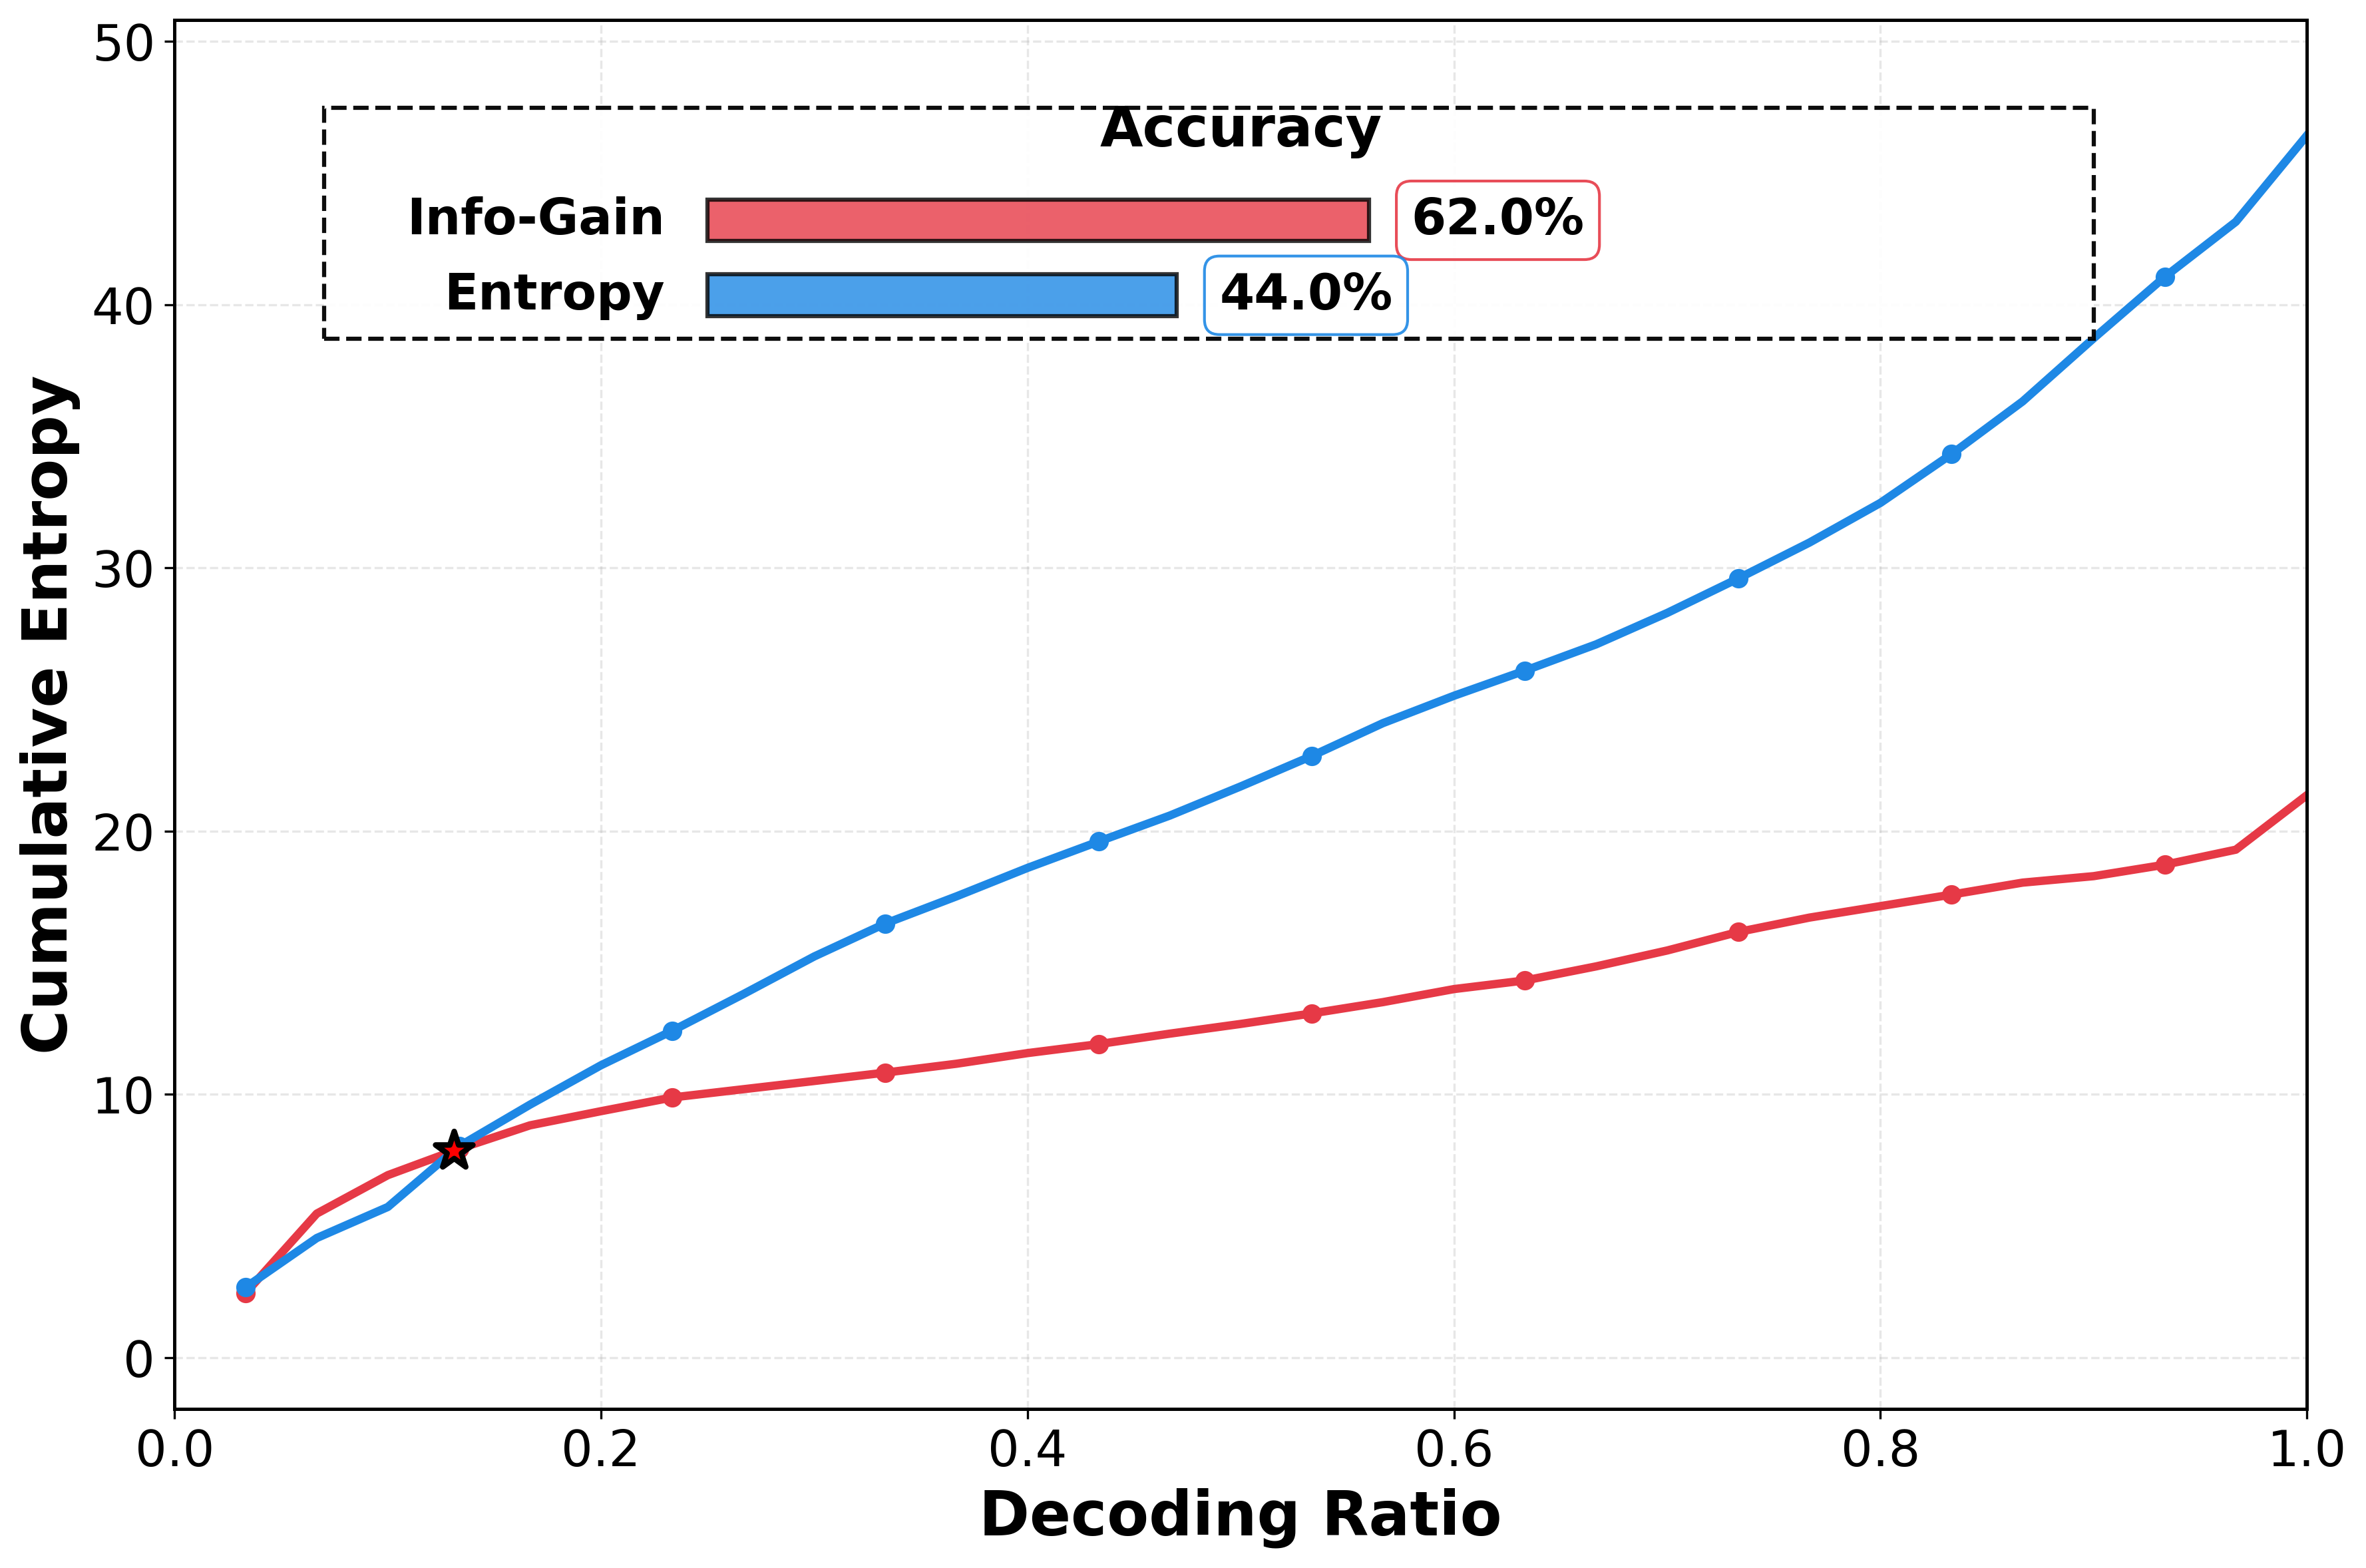
\includegraphics[width=\linewidth]{abla-1.png}
        \caption{Cumulative entropy trajectories}
        \label{fig:abla_entropy}
    \end{subfigure}
    \hfill
    \begin{subfigure}[b]{0.5\textwidth}
        \centering
        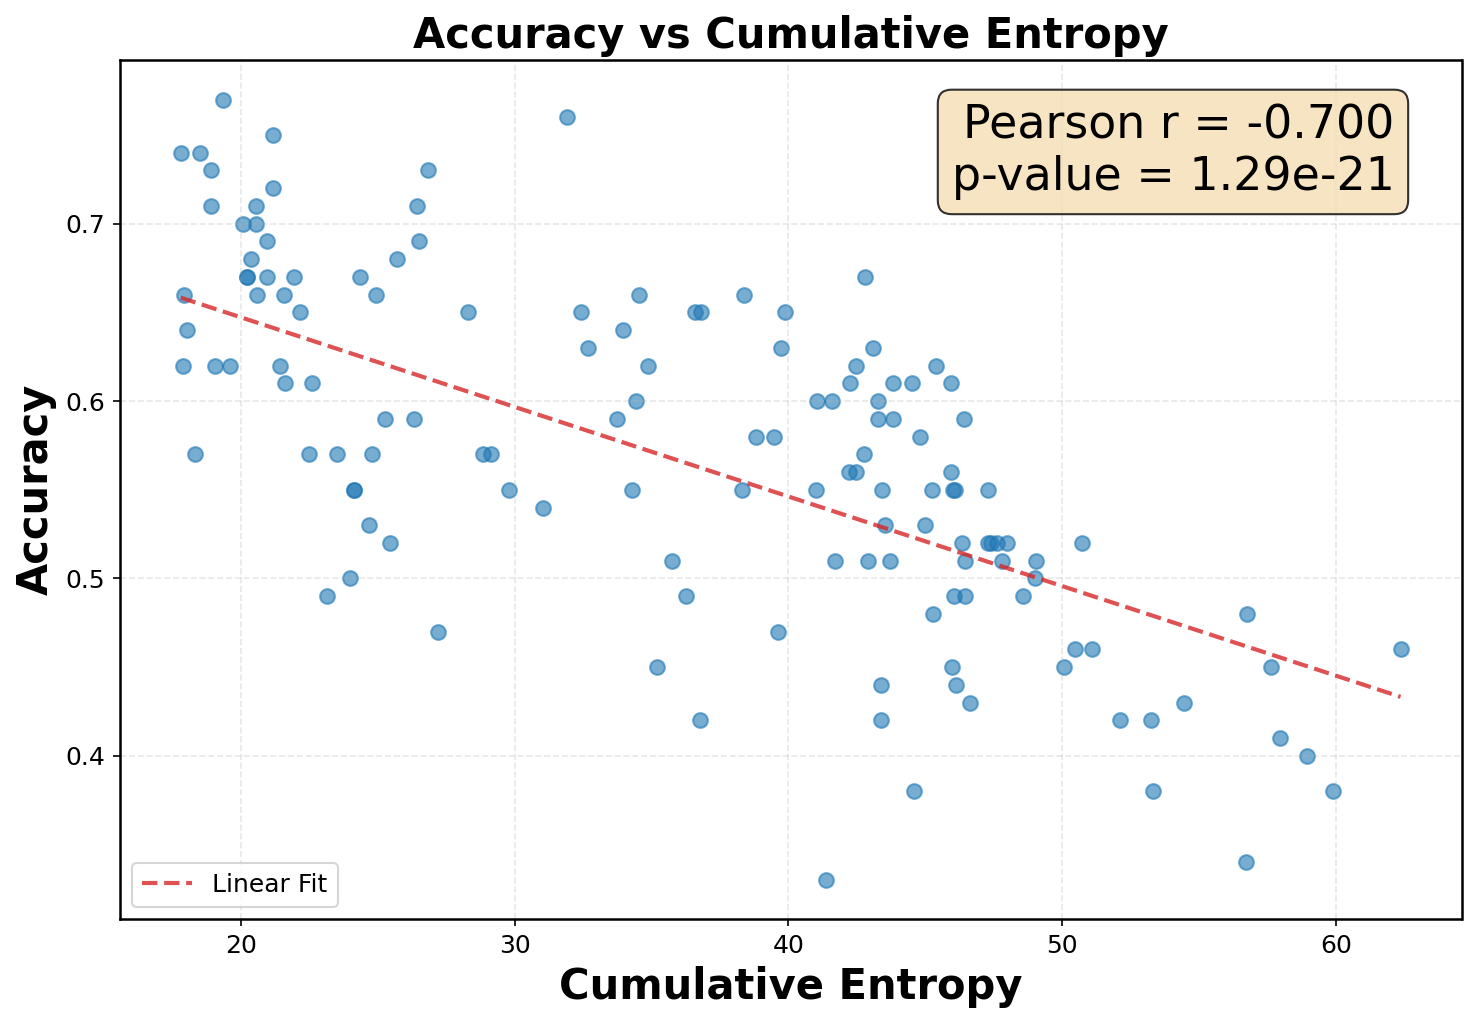
\includegraphics[width=0.98\linewidth]{abla-4.png}
        \caption{Accuracy vs. Cumulative Entropy}
        \label{fig:ent vs acc}
    \end{subfigure}
    \caption{\textbf{Analysis of Cumulative Entropy.} (a) Cumulative entropy trajectories for the Entropy baseline and Info-Gain Sampler on a synthetic set of 100 simple arithmetic problems that can be answered within a short window. We use global decoding with a fixed length of 64 tokens. (b) Correlation between average accuracy and average cumulative entropy across various sampling configurations.}
    \label{fig:entropy_analysis}
\end{figure}

\begin{figure}[!h]
\centering
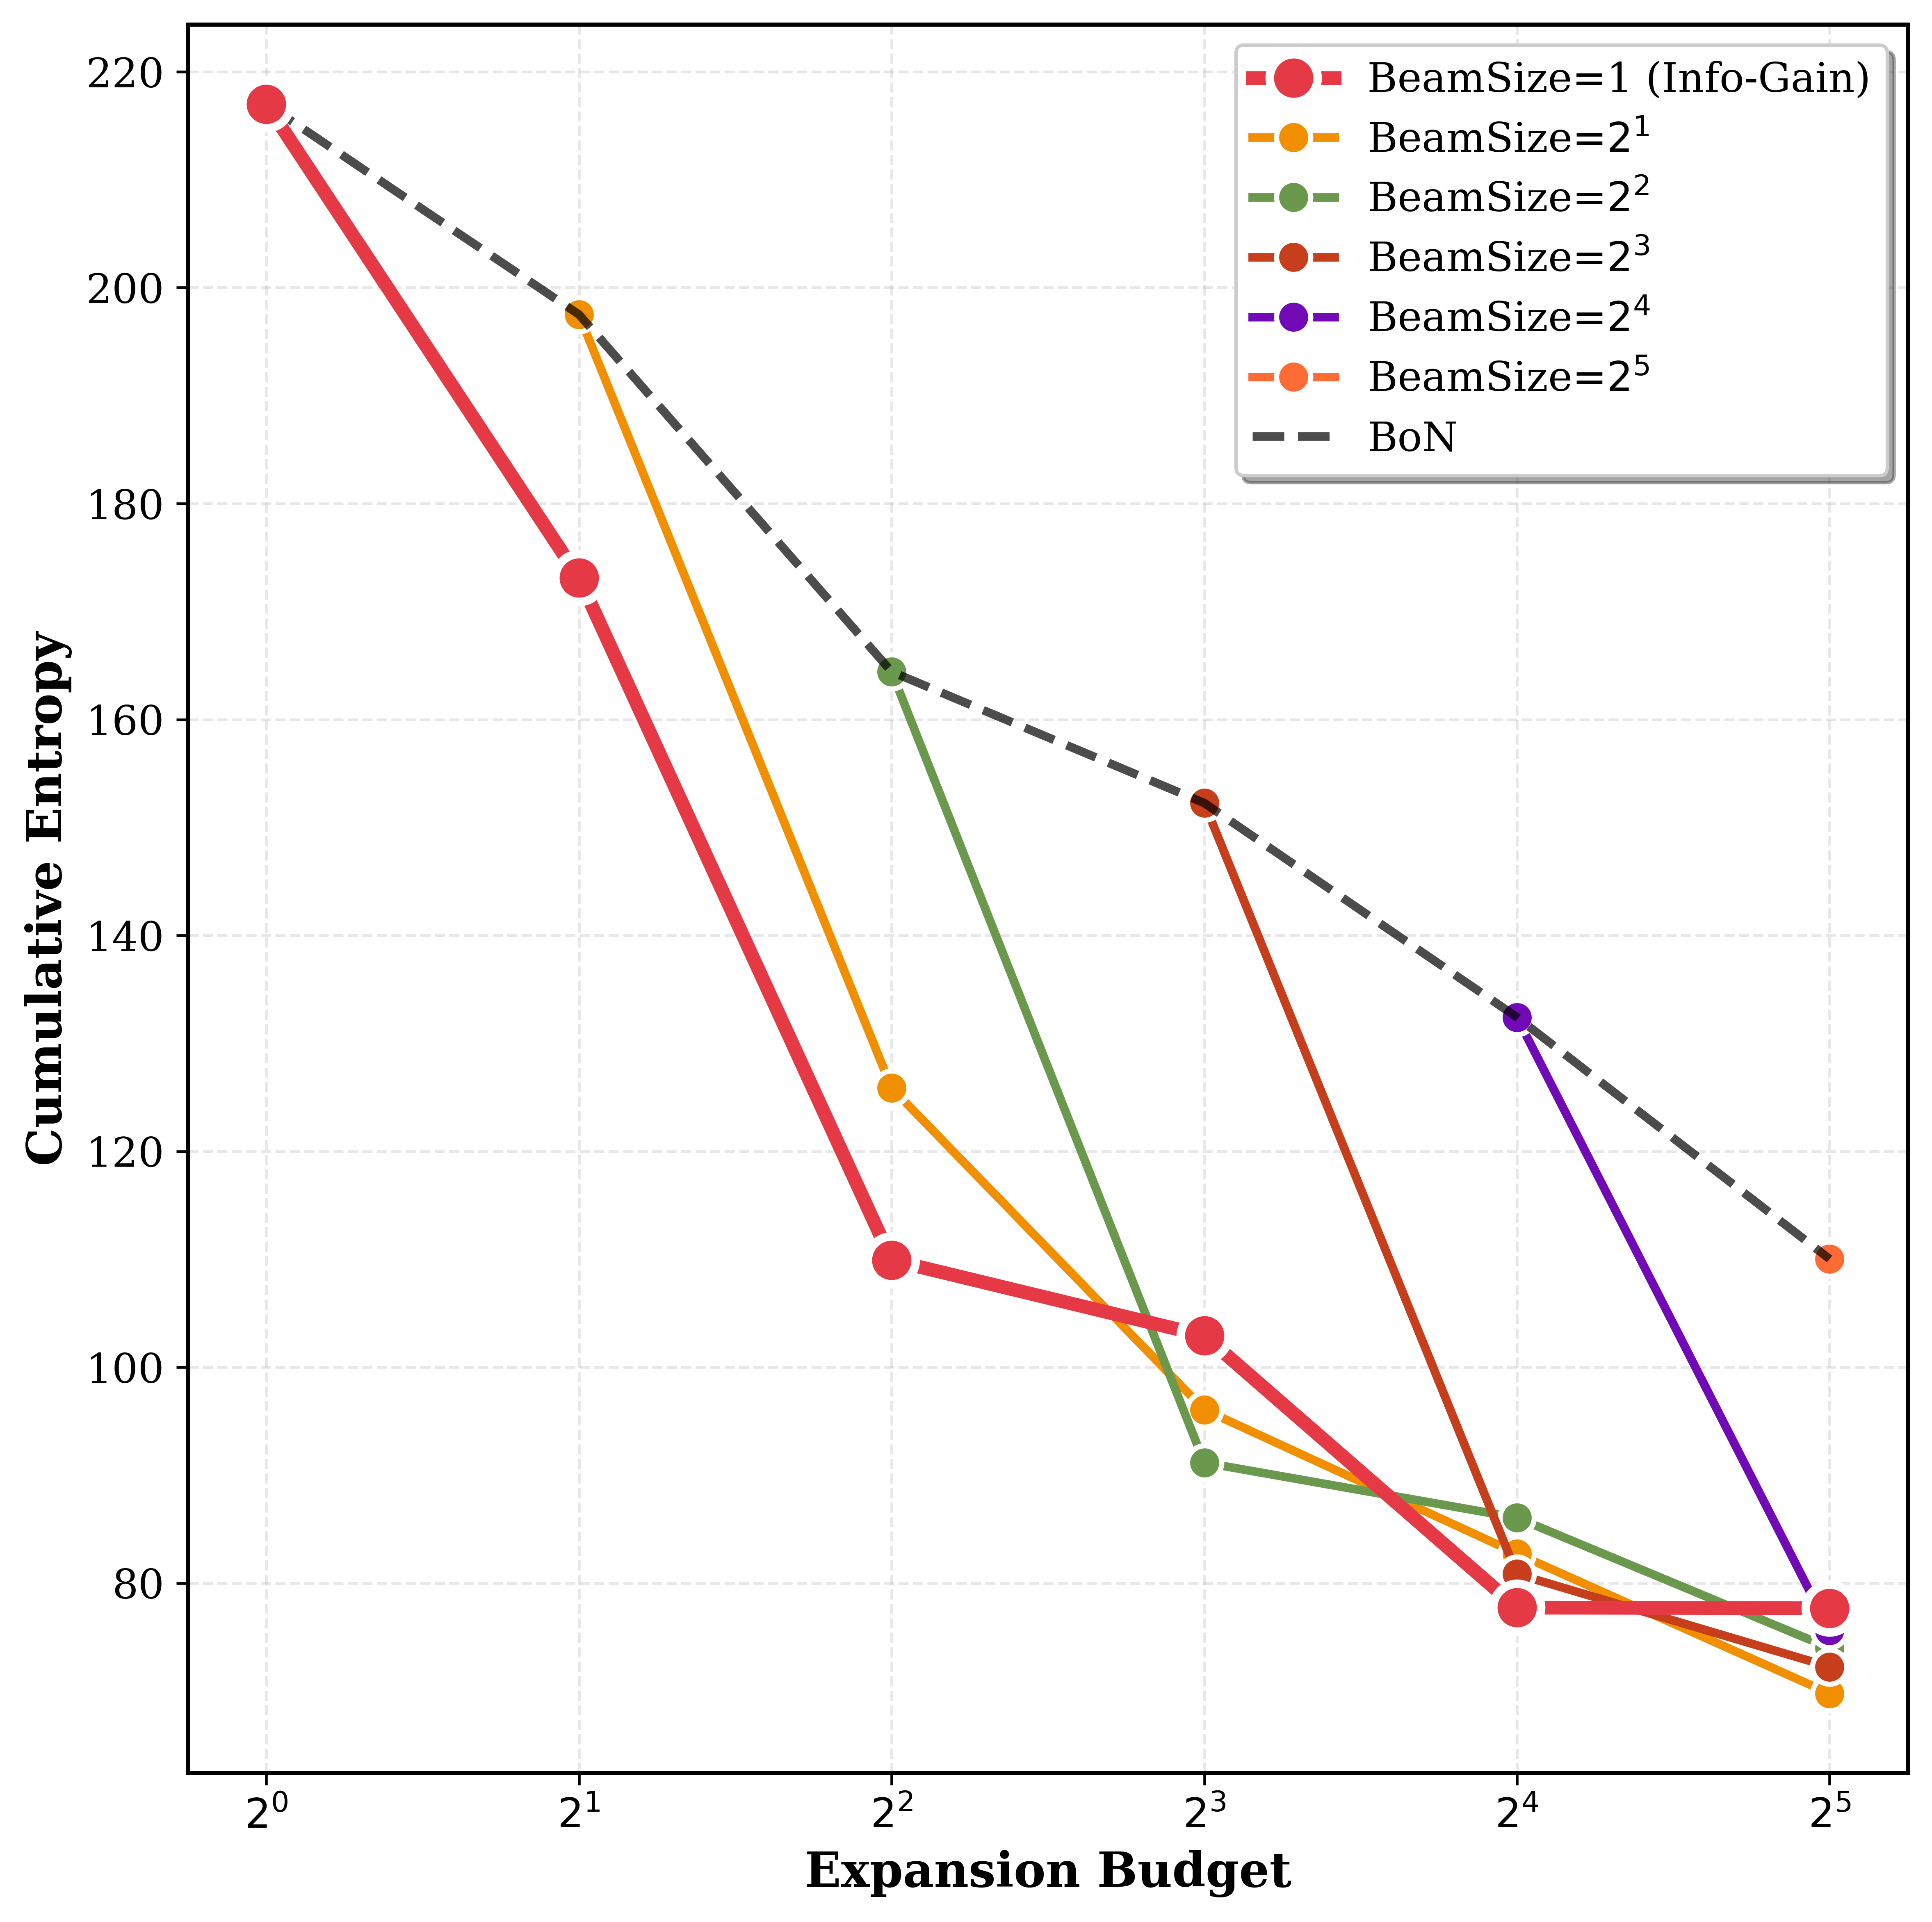
\includegraphics[width=0.80\linewidth]{abla-2.png}
\vspace{-1mm}
    \caption{Impact of different beam sizes on the MATH-500 dataset. Specifically: \textbf{Beam Size = 1} is a special case equivalent to the Info-Gain Sampler; \textbf{Beam Size = Expansion Budget} is equivalent to the Best-of-$N$ (BoN) baseline; and \textbf{Intermediate Values} represent a look-ahead beam search algorithm using Info-Gain as the pruning heuristic.}
    \label{fig:budget_ablation}
\end{figure}
\begin{figure}[!h]
    \centering
    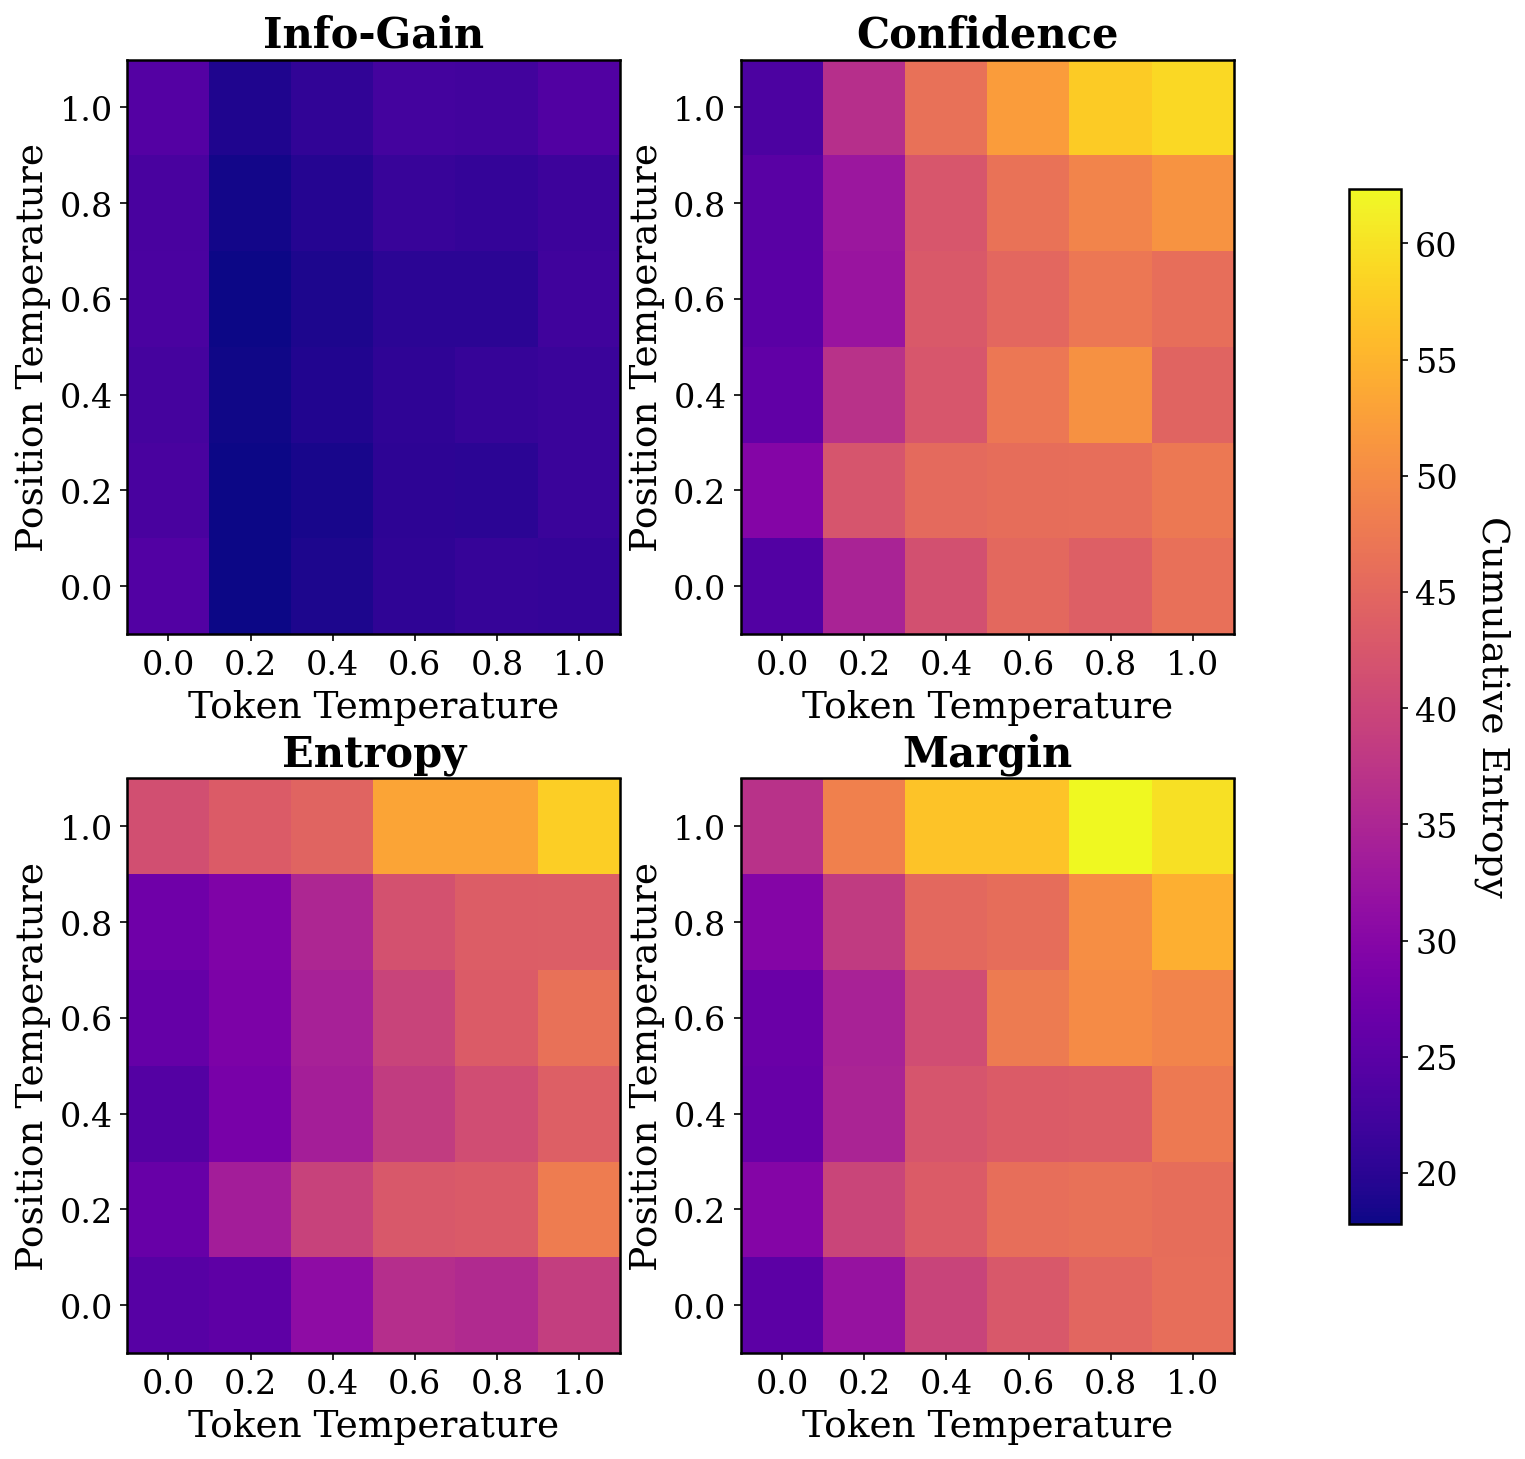
\includegraphics[width=1\linewidth]{entropy-vs-temperature.png}
    \vspace{-4mm}
    \caption{\textbf{Temperature Sensitivity.} Cumulative trajectory uncertainty under varying position and token temperatures on the 100 simple arithmetic problems, evaluated using global decoding with a fixed length of 64 tokens.}
    \label{fig:temperature-entropy}
\end{figure}
\subsection{Ablation Study}
\vspace{-1mm}
\noindent\textbf{Optimization of Cumulative Uncertainty.}
As shown in Table~\ref{tab:dream_results}, the \textbf{Info-Gain Sampler} significantly outperforms baselines in optimizing cumulative uncertainty. By tracking cumulative entropy during decoding on mathematical reasoning tasks (Fig.~\ref{fig:entropy_analysis}), we observe that:
(1) The Info-Gain heuristic balances immediate cost with future gains, yielding non-linear entropy growth that stabilizes earlier than the greedy Entropy baseline.
(2) Cumulative entropy shows a strong \textbf{negative correlation with accuracy} (Pearson's $r=-0.70$), validating it as a reliable proxy for decoding quality.

\noindent\textbf{Comparison of Info-Gain Variants.}
We compare the \textbf{Info-Gain Sampler} ($B=1$), \textbf{Info-Gain Beam Search} ($B>1$), and \textbf{Best-of-N (BoN)} under a fixed computational budget (Figure~\ref{fig:budget_ablation}). For beam search variants, we adopt the following configuration: the beam width is set to $B$, and the scoring function is defined as the sum of cumulative entropy and state uncertainty. The decoding process terminates when all hypotheses in the beam have been fully decoded.
(1) The \textbf{Info-Gain Sampler ($B=1$)} performs near the Pareto frontier, achieving near-optimal results while remaining highly parallelizable and avoiding complex KV-cache management.
(2) Both Info-Gain variants significantly outperform \textbf{BoN}, proving that global planning via information gain is superior to simply increasing independent samples.
(3) Increasing \textbf{Beam Size} under given expansion budget yields marginal uncertainty reduction but incurs higher memory overhead (Appendix~\ref{appendix:memory}).

\noindent\textbf{Compatibility with Temperature Sampling.} 
We investigate the impact of position and token temperature settings on cumulative uncertainty. For the baselines, the position temperature mechanism is implemented by applying a softmax with temperature to the heuristic scores followed by categorical sampling, where a position temperature of zero corresponds to the original greedy sampling.
As shown in Figure~\ref{fig:temperature-entropy}, the Info-Gain Sampler maintains stable, low trajectory uncertainty across various temperature scales without sensitive tuning. Importantly, low cumulative entropy reflects more optimized decoding rather than mode collapse, as evidenced by the preserved diversity and competitive win rates in creative writing (Table~\ref{tab:creative_writing}). In contrast, other baselines are highly sensitive to temperature changes, leading to decoding instability. 